\chapter{Design} \label{cha:design}
	This chapter explains the design of the system. This includes: back-end
	design, model/graphical design, and main activities.

	\section{Main activities} \label{sec:mainactivities}
		There are several main activities in the system, corresponding to the two
		main user types of the system. These user types are both the physically co-
		located	players as well as the physically remote players. The activities
		are as follows:

		\subsection{A local user wants to start a game} \label{ssec:userstartgame}
			The local user ensures the main camera is set up according to the 
			provided guidelines. The local user then starts the server on the 
			machine the camera is connected to. The local user needs to take note 
			of the IP address of the server machine and fill this into his local 
			machine (to which the Meta One glasses are attached). The other players
			also fill in the same IP address. The server can also run on one of the 
			players' machines. The local user needs to wait for others to join the 
			game. When at least two local players and at least one remote player 
			has joined the game, the game will start.
			
		\subsection{A local user wants to join a game} \label{ssec:localjoingame}
			A local player wants to join an active game. Before this can
			happen, a game has to be started first. The local player needs to 
			acquire the IP address of the server machine and fill this in.
			Once the game starts, the local player will see virtual objects projected 
			through the Meta One glasses.

		\subsection{A remote user wants to join a game} \label{ssec:remotejoingame}
			A physically remote player wants to join an active game. Before this can
			happen, a game has to be started first. The remote user needs to acquire 
			the IP address of the local server machine (see \ref{ssec:userstartgame})
			and fill this in. The remote user will see a virtualized version of the 
			same game world as the local players.
			
		\subsection{A local player wants to move a mirror} \label{ssec:localmovemirror}
			A local player is partaking in an active game. To hit the target, they
			need to move a mirror from point A to point B to allow the laser beam
			coming from the emitter to be deflected and therefore to hit the target.
			The local player uses moveable markers to place a mirror in the game
			world. Using the Meta One glasses, local players can see the game objects
			when they see a marker. For this example, it is assumed that the player that wants
			to move the mirror marker also has that mirror marker to their disposal,
			and also that the mirror is rotated such that no more rotation is required.
			The local player can then take the mirror marker, move it to the point
			it should be moved to, and complete the game that way.
			
		\subsection{Two local players want to move a mirror} \label{ssec:localmovemirrorcollab}
			Due to mirror markers being divided between the players, it is possible
			that two (or, more generally speaking, multiple) players want to move
			a mirror, possibly the last mirror required to solve the level. However,
			a mirror marker can only be placed by one person. The local players then
			need to collaborate on where the marker should be placed. As the players
			are physically co-located (by definition of them being local players),
			this collaboration can happen in multiple ways, like pointing to a 
			location on the playing field, or discussing the best position for the
			marker.
			
		\subsection{A remote player wants to rotate a mirror}
			Remote players, due to them not being physically co-located with the
			local players, cannot move mirror markers, as that would require them
			to meet up with the local players and to play with them. However, 
			remote players have access to an ability that the local players do
			not have access to, that being the ability to rotate selected mirrors.
			The remote player uses a computer for this. In order to rotate a mirror,
			the player has select a mirror first. Using the "M" key, the player can
			cycle through mirrors, but they can also click on a mirror in the game
			world to select that mirror. When a mirror is selected, the outer
			frame of the mirror (shown in \ref{fig:mirror}) will change color
			from gold to bright yellow, indicating that this mirror is selected
			(the recolor will only be visible for the remote player responsible
			for clicking on that mirror, even other remote players will not be
			able to see this recolor). Also, a selected mirror can be rotated by
			using the "A" key (for rotation to the left, relative to the surface
			normal of the mirror) or the "D" key (for rotation to the right).
			
		% TODO add some use case diagrams?

	\section{Back-end design} \label{sec:backenddesign}
		The system is composed of three main parts: The Laser mechanics, the network
		functionality and the projection to 3D glasses. For this purpose, we divided
		the C\# code over three namespaces, named "Core", "Network" and
		"Projection", respectively.

		The "Core" namespace is responsible for drawing the Laser beams and
		providing the interactions of laser beams with the other game objects.
		The layout of this namespace is discussed in paragraph 
		\ref{ssec:corenamespace}.

		The "Network" namespace is responsible for synchronizing the game state
		between all connected players. The layout of this namespace if discussed 
		in paragraph \ref{ssec:networknamespace}.

		The "Projection" namespace is responsible for providing the projection to
		the VR glasses. This namespace provides the functionality required to project
		the game world to the VR glasses. The layout of this namespace is discussed in
		paragraph \ref{ssec:projectionnamespace}.
		
		Additionally, the game depends on the deployment of a server application written
		in C++. The purpose of this server application will be discussed in
		\ref{ssec:networknamespace}.
		
		\subsection{The Core namespace} \label{ssec:corenamespace}
			%TODO: Write about core namespace.
			%      Also include the class diagram.
			
		\subsection{The Network namespace} \label{ssec:networknamespace}
			The Network namespace has undergone several changes since the start
			of the project. These changes are described in this part.
			
			The first take on creating a network functionality in the game
			was to use the standard way of networking within Unity itself.
			This involved creating a rather simple networking script that
			allowed the game to connect to the Unity master server or their own
			master server (provided they had one installed), which then handled
			all changes that were recorded by network view components of objects,
			and sent them to all the players, synchronizing the game world.
			There are several tutorials on how to write such a networking
			script and how to use it in a multiplayer game, the tutorial that
			was used for the script in the namespace can be found here:
			\url{http://www.paladinstudios.com/2013/07/10/how-to-create-an-online-multiplayer-game-with-unity/}
			
			The base networking functionality of Unity, however, was not enough
			for what we were trying to do (for example, it had very poor VR and
			AR support, and our game is an AR game after all). Because of this,
			a different solution was required to create synchronization across
			the game world. The next option was to use the Photon Unity Networking
			package, which not only supported multiplayer better (it allowed for
			more people to play the same game), but it also allowed VR and AR games
			to have multiplayer functionality (there is a free package available
			on the Unity Asset Store, which can be found here: \url{https://www.assetstore.unity3d.com/en/#!/content/1786}). However,
			this was not used, as the problem was not that we needed to connect
			several AR players in the game world (as these would be the local players,
			and therefore would be able to see what was going on in the game world
			by just looking at the marker that was placed near them). As such,
			a different solution had to be found.
			
			The final solution is the solution that is used right now. 
			%TODO: Check this part, and write about OpenCV.
			%      Also include the class diagram and a piece about the OpenCV server.
					
		\subsection{The Projection namespace} \label{ssec:projectionnamespace}
			%TODO: Write about projection namespace.
			%      Also include the class diagram.

	\section{Game elements} \label{sec:graphicaldesign}
		For designing the 3D models, we used Blender. Blender is a free application
		for 3D modeling, under the GPL license, and Unity natively support Blender 
		models (provided Blender is installed on the system). We have chosen for a 
		light looking style featuring nature inspired modeling and gold and crystal 
		based materials. The light modeling style causes slight miss alignments with 
		the ground to be less noticeable and makes the lack of feedback from moving a 
		card feel less odd. The crystals and gold just feels good in combination with 
		the beams of light.
		
		The following sections display and describe the graphics used in
		the gameplay elements, as well as the function of
		these elements.
		% TODO Explain why we chose this graphics style
		
		\subsection{Laser target} \label{ssec:lasertarget}
			The laser target is the main target of the game. It consists of
			a small container, which contains a crystal. The point of the
			game is to direct a laser beam from an emitter to this target.
			When the target is hit by a laser beam, the outer columns around
			the crystal inside will rotate and spread out, indicating that
			the target has been hit. The game will then proceed to the
			next level. An image of the target is shown in figure 
			\ref{fig:target}.
			\begin{figure}[h]
				\centering
				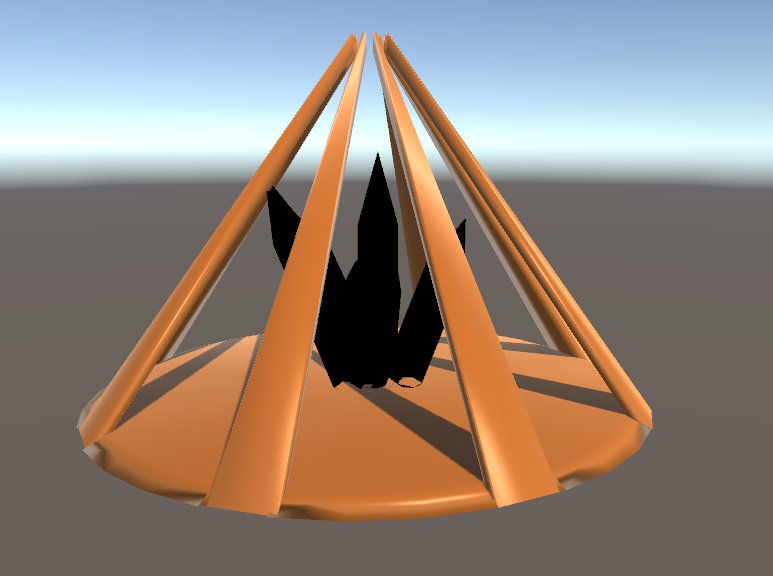
\includegraphics[scale = 0.4]{Target}
				\caption{The target of the game. The gold columns around the inner crystal will open up and rotate once the target is hit, as described earlier. Also, the crystal will change color once the target hits it.}
				\label{fig:target}
			\end{figure}
			
		\subsection{Mirror} \label{ssec:mirror}
			A mirror is a crucial game element. Its reflective surfaces
			allow it to reflect any laser beam that hits these surfaces.
			It is also the only element that players can move and/or rotate.
			All levels require at least one mirror to move or rotate
			in order to hit the target. An image of a mirror in-game is shown
			in \ref{fig:mirror}.
			\begin{figure}[h]
				\centering
				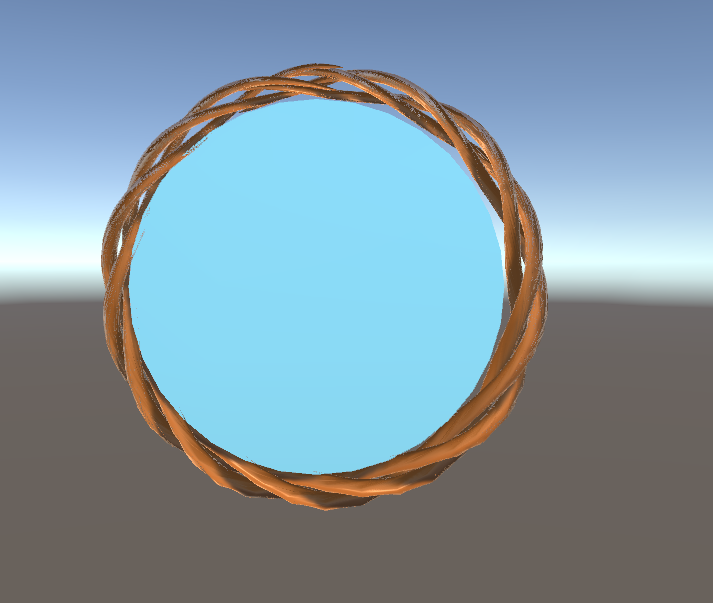
\includegraphics[scale = 0.3]{Mirror}
				\caption{an image of a mirror in-game, with its reflective surfaces.
				The light blue circles reflect laser beams, the golden outer frame
				does not.}
				\label{fig:mirror}
			\end{figure}
			
		\subsection{Wall} \label{ssec:wall}
			The wall is the main obstacle in the game. It blocks incoming
			laser beams completely. Walls are used in levels to make it 
			less easy for one player to reflect a laser beam coming from
			an emitter to the target. The first few levels mainly use walls
			to create paths that the laser beam has to go through, later
			levels use not only walls, but also other game objects. A wall
			is shown in \ref{fig:wall}.
			\begin{figure}[h]
				\centering
				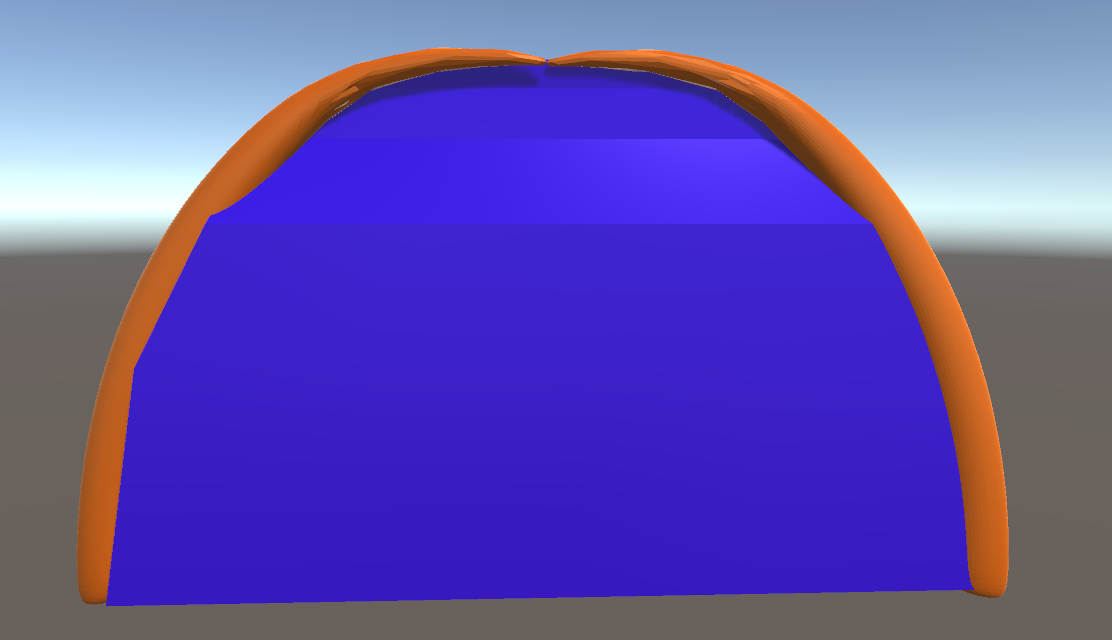
\includegraphics[scale = 0.15]{Wall}
				\caption{an image of a wall in-game. It blocks lasers entirely.}
				\label{fig:wall}
			\end{figure}
			
		\subsection{Emitter} \label{ssec:emitter}
			The emitter is the most important aspect of the entire game.
			It is the only "true" source of a laser beam (although game
			elements like the beam splitter can also create beams, these
			elements always require input in the form of another laser
			beam; the emitter does not have that problem, hence it is a "true"
			source). In the early levels, players only move and rotate mirrors
			to guide a laser beam from the emitter to the target, while in the
			later levels beams have to be guided towards other game elements
			(like the beam splitter, for example) in order to complete the
			level. It is possible to have multiple emitters in a single level,
			and later levels use this to create more complex puzzles.
			What the emitter looks like exactly is shown in figure 
			\ref{fig:emitter}.
			\begin{figure}[h]
				\centering
				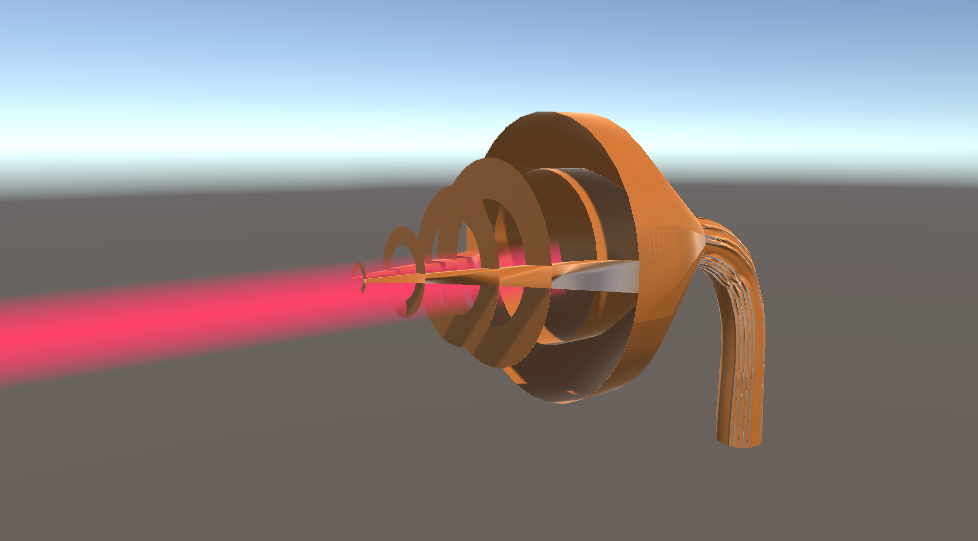
\includegraphics[scale = 0.25]{Emitter}
				\caption{what the emitter looks like in the game. Also shown here is a laser beam
				coming from the emitter. The laser beam is colored red per standard. There are game objects that can change the coloring of the beam, these will also be described in this part of the report.}
				\label{fig:emitter}
			\end{figure}
			
		\subsection{Elevator} \label{ssec:elevator}
			The elevator is a game object that uses mirrors to elevate laser beams
			to a new height. This then allows laser beams to pass over walls that 
			stand on the ground. Therefore, elevators can function as a bridge over
			walls. An elevator is depicted in \ref{fig:elevator}.
			\begin{figure}[h!]
				\centering
				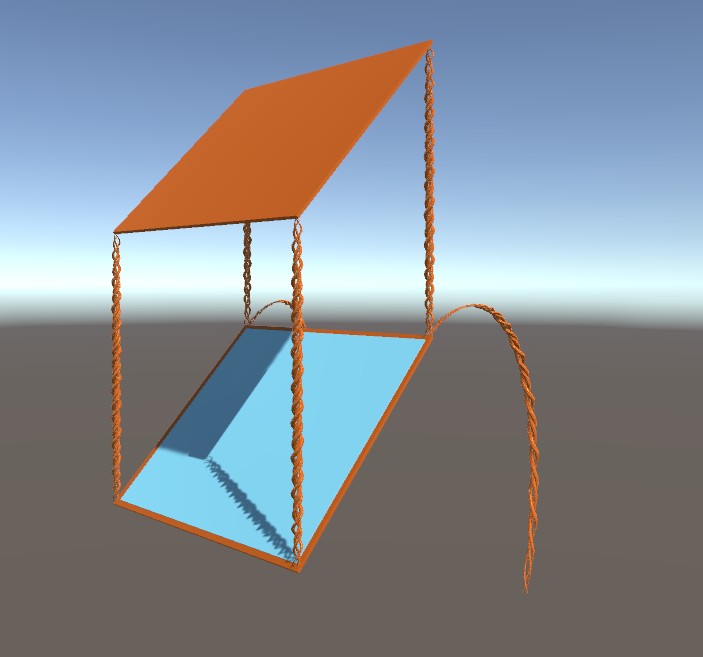
\includegraphics[scale = 0.3]{Elevator}
				\caption{an elevator in-game. Both the upper and lower plate have a
				mirror (represented on the bottom plate as a light blue plate),
				which reflects laser beams.}
				\label{fig:elevator}
			\end{figure}
		\subsection{Portal}
			The portal is a more advanced game object. It allows light that travels 
			into it to travel out of the portal it is linked to, and vice versa. This
			allows puzzles to contain targets that cannot be hit by just reflecting
			laser beams from the emitters by mirrors (as the laser beams have to
			travel through a portal in order to be able to hit the target),
			therefore forcing the players to redirect laser beams to portals.
		\subsection{Lens splitter}